\documentclass[12pt]{article}
\usepackage{amsmath,amssymb,graphicx}
\begin{document}

\section*{Simple GAN Implementation}

\subsection*{Generative Adversarial Networks}

\indent The code is a very simple interpretation of a generative adversarial network, a very recent machine learning model. While neural networks are traditionally discriminative models, generative adversarial nets were proposed as a way of training a neural network to learn a data distribution.

The structure revolves around having a generator that starts by producing random noise. The discriminator network is trained to differentiate between data points sampled from the actual and generated distribution. The generator is trained to produce data points that will trick the discriminator (i.e. probability of correct classification is 0.5). The scenario is a minimax game where the discriminator attempts to maximize the proportion of successful classifications while the generator attempts to minimize the proportion of successful classifications.
$$ \underset{G}{min} \underset{D}{max} J(D,G)=\mathbb{E}_{\textbf{x}\sim p_{data}(x)}[log(D(\textbf{x}))]+\mathbb{E}_{\textbf{z}\sim p_{g}(z)}[log(1-D(G(\textbf{z})))]$$
$D(x)$ is probability the discriminator identifies $x$ from the true distribution\\
$G(z)$ is the generator's transformation on the input noise

\subsection*{Tools}
\indent The implementation uses Python 2.7. Numpy and Tensorflow are used as for data structures, matrix operations, and machine learning tools. Matplotlib and seaborn are used for basic data visualization.

\subsection*{Implementation}
This implementation is based off a Paperspace GAN tutorial\cite{Paperspace Blog}.\\
User controlled parameters (help available through the --help argument) include: number of hidden layers and width of each layer for the discriminator and generator networks, number of iterations to train the generator, amount of iterations to train the discriminator between each generator update, and batch size.

\subsubsection*{Generator and Discriminator Structure}
The generator and discriminator is a deep feedforward network uses the leaky relu activation function:
$$ f(x)=max\{\alpha x, x\} $$
Tensorflow uses a default value of $\alpha=0.2$. The number and width of generator and discriminator hidden layers are set to $[10,10,10]$ by default, but changable as a user argument.

\subsubsection*{Generator and Discriminator Interaction}
The discriminator must be optimized to differentiate between true and generated data before each update to the generator's weights. As a result, it may be necessary to adjust the number of iterations used to optimize the discriminator (defined as the $k$-ratio in the original paper). The default setting updates the discriminator with 20 iterations before updating the generator. The default batch size is set to 100.

\subsubsection*{Loss Function}
The cost function used is the sigmoid cross-entropy logit function. This is just a composition of the cross entropy loss function onto the sigmoid of the prediction.
$$J(\hat{y},y)=y*-log(sigmoid(\hat{y}))+(1-y)(-log(1-sigmoid(\hat{y})))$$
$$=y*-log(\frac{1}{1+e^{\hat{y}}})+(1-y)*(-log(1-\frac{1}{1+e^{\hat{y}}}))$$
where $y$ is the label and $\hat{y}$ is discriminator prediction

\subsubsection*{Optimization Methods}
It also uses a common adaptive learning rate technique, RMSProp, during gradient descent. RMSProp uses an exponentially decaying average of squared gradients to control the rate of descent - the effect of using RMSProp is that rate of descent decays in directions where the gradient consistently decreases or changes signs. The decay rate, $\gamma$, is set to 0.9 by default in TensorFlow. Momentum is disabled by default. $\epsilon$ is just a small constant used to avoid divide-by-zero errors and is set to $1\mathrm{e}{-10}$ by default. The learning rate, $\eta$, used in the tutorial is $0.001$.
$$r_t=\gamma r_{t-1}+(1-\gamma)(\nabla_w J)^2_t$$
$$\Theta_{t+1}=\Theta_{t}-\frac{\eta}{\sqrt{r^2_t+\epsilon}}\nabla_w J$$

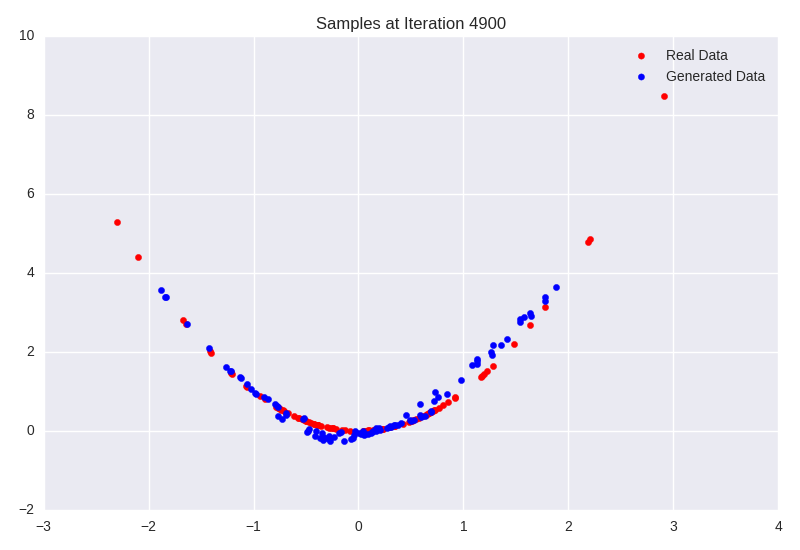
\includegraphics[scale=0.5]{../iterations/iteration_4900.png}\\
Sample output with true distribution mimicing a parabola, all settings set to default.

\begin{thebibliography}{9}
\bibitem{Paperspace Blog}
GAN Tensorflow Implementation
\\\texttt{https://blog.paperspace.com/implementing-gans-in-tensorflow/}
\end{thebibliography}
\end{document}